\documentclass[12pt,a4paper]{article}
%\usepackage[cp1251]{inputenc} 
%\usepackage[T2B]{fontenc}     
%\usepackage[russian]{babel}
%\usepackage[T1]{fontenc}
\usepackage{iftex}
\ifTUTeX
  \usepackage{fontspec}
\else
  \usepackage[T1]{fontenc}
  \usepackage[utf8]{inputenc} % The default since 2018
  \DeclareUnicodeCharacter{200B}{{\hskip 0pt}}
\fi
\usepackage{multirow} 
\usepackage{enumitem}
\usepackage{graphicx}
\usepackage{xcolor}
\usepackage{array}
\usepackage{booktabs}
\usepackage{amsmath}

\DeclareGraphicsExtensions{.pdf,.png,.jpg}   
\newcolumntype{P}[1]{>{\centering\arraybackslash}p{#1}}
\newcolumntype{M}[1]{>{\centering\arraybackslash}m{#1}}
\begin{document}
\title{HW3 - Theory questions}
\author{Valeriia Kravchik - 342390093}
\date{\today}
\maketitle
%-----------------------------------------------------------------------------------------------------------------
\newpage
\begin{center}
\textbf{Q1 - Clustering}
\end{center}
\begin{enumerate}[label=(\alph*)]
\item Note that the K-means algorithm is quite sensitive to noise and unnecessary data (outliers), since it is usually quite strongly influenced by extreme values. At the same time, a rather similar K-medoids algorithm, which is essentially a variant of K-means, is much more reliable in relation to noise and outliers.\cite{Mannor2011}\\
K-means clustering assignes each point to the cluster whose center is nearest. The center of the cluster is defined as the average of all points in the cluster. The algorithm attempts to minimize the intra-cluster variance defined by\cite{Lloyd}:
$$
\displaystyle V = \sum_{i=1}^{k}\sum_{x_j \in S_i}\left(x_j - \mu_i\right)^2
$$
where there are $k$ clusters $S_i, i = 1,2,\dots,k$ and $\mu_i$ is the center of all points $x_j \in S_i$.\\
K-medoids clustering is computed using the PAM-algorithm (PAM is short for Partitioning Around Medoids). It chooses datapoints as centers in contrast to the K-means algorithm. The PAM-algorithm is based on the search for $k$ representetives (called medoids) among all elements of the dataset.When having found $ k$ representatives $ k$ clusters are now generated by assigning each element to its nearest medoid.Then it finds a local minimum for the objective function\cite{Kaufman}:
$$
\displaystyle V = \sum_{i=1}^{k}\sum_{x_j \in S_i}\left(x_j - c_i\right)^2
$$
where there are $k$ clusters $S_i, i = 1,2,\dots,k$ and $c_i$ is the medoid of $ S_i$.
So we know that the K-means uses a sum of squared Euclidean distances for minimization. But we know that K-medoids method tries to minimize a sum of pairwise dissimilarities. Little reminding about Euclidean distance between $ u$ and $ v$. It is:
$$
\displaystyle \vert u-v\vert = \sqrt{\sum_{i=1}^n (u_i-v_i)^2} 
$$
Let me visualize a robustness of K-medoid, when working with noise:\\
Consider a dataset of 5  points in 2D (Figure \ref{ris:K}):\\ (1,1),(1,2),(2,1),(2,2)(3,3):\\
\begin{figure}[h]
\center{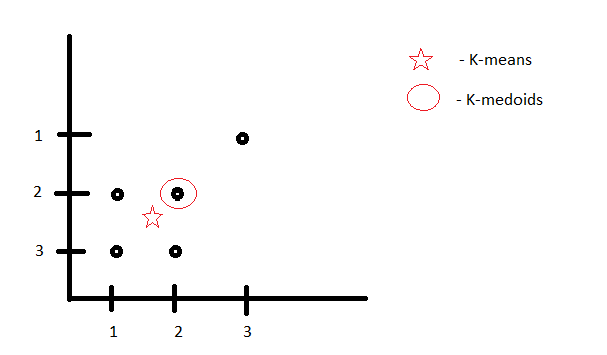
\includegraphics[scale =1]{K}}
\caption{K-means vs K-medoids}
\label{ris:K}
\end{figure}
Center of data using K-means:\\
$$
\displaystyle X_{mean} = \frac{1+1+2+2+3}{5} = 1.8 
$$
$$
\displaystyle Y_{mean} = \frac{1+1+2+2+3}{5} = 1.8 
$$
For K-medoids center of data. We need to arrange $X_i$ in ascending order = 1,1,2,2,3, and from here the median is the middle for, that is 2. The same for $Y_i$, the medoid = 2 (Figure \ref{ris:K}).\\
Let us to produce the outlier in point (100,100) (Figure \ref{ris:K1}):
\begin{figure}[h]
	\center{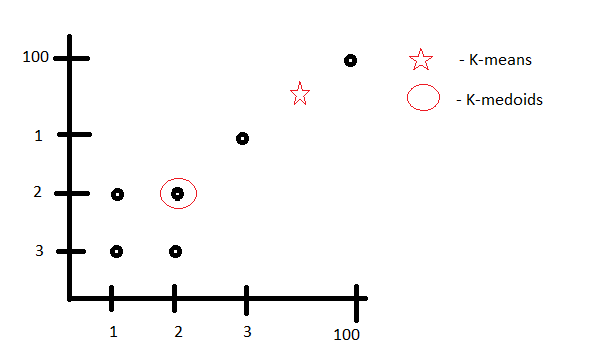
\includegraphics[scale =1]{K1}}
	\caption{K-means vs K-medoids with outlier}
	\label{ris:K1}
\end{figure}

Center of data using K-means:\\
$$
\displaystyle X_{mean} = \frac{1+1+2+2+3+100}{6} = 18.16 
$$
$$
\displaystyle Y_{mean} = \frac{1+1+2+2+3+100}{6} = 18.16  
$$
For K-medoids center of data. We need to arrange $X_i$ in ascending order = 1,1,2,2,3,100.\\
$$
\displaystyle X_{median} = average~ of (\frac{n}{2}term+\frac{n+1}{2}term) = \frac{2+2}{2}=2
$$ 
We need to arrange $Y_i$ in ascending order = 1,1,2,2,3,100.\\
$$
\displaystyle Y_{median} = average~ of (\frac{n}{2}term+\frac{n+1}{2}term) = \frac{2+2}{2}=2
$$ 
We can pay attention that after adding the outlier the center for K-means moved from (1.8,1.8) to (18.16,18.16). But the K-medoids is still the same! Thus we can say that K-medoids algorithm is more  robust to outliers and noise than K-means algorithm.

\item Let $z = \sum_{i=1}^{n}\left(x_i - \mu \right)^2  $ for any $\mu$\\
From the maxima minima principle we know, that $z$ has it's minimum when:
$$
\displaystyle \frac{\partial z}{\partial \mu} = 0 ~ and ~ \frac{\partial^2 z}{\partial^2 \mu} > 0
$$$$
\displaystyle \frac{\partial z}{\partial \mu} = \frac{\partial}{\partial \mu}\left[ \sum_i x_i^2 - 2\mu \sum_i x_i + \sum_i \mu^2 \right] = 
$$$$
\displaystyle =  \frac{\partial}{\partial \mu}\left[ \sum_i x_i^2 - 2\mu \sum_i x_i + n \mu^2 \right] = 0 - 2\sum_i x_i +2n\mu
$$
from $\frac{\partial z}{\partial \mu} = 0$
$$
\displaystyle \Longrightarrow  -2\sum_i x_i +2n\mu = 0
$$
$$
\displaystyle \Longrightarrow  -\sum_i x_i +n\mu = 0
$$
$$
\displaystyle \Longrightarrow  \mu =\frac{1}{n} \sum_i x_i 
$$

For $\mu =\frac{1}{n} \sum_i x_i $, $\frac{\partial^2 z}{\partial^2 \mu} = 2n > 0$\\[5pt]
$z$ is minimized at $\mu =\frac{1}{n} \sum_i x_i $\\[5pt]
Hence, $\mu =argmin_\mu\sum_i \left(x_i -\mu \right)^2$



\item[\textbf{Bonus}] Let $z = \sum_{i=1}^{n}\vert x_i - \mu \vert$\\[5pt]
set arrange $x_i^s$ such that $x_1<x_2<\dots<x_n$\\[5pt]
for $\mu \in set[x_1,x_n]$ we get:
$$
\displaystyle \sum_{i=1}^{n}\vert x_i - \mu \vert = \sum_{i=2}^{n-1}\vert x_i - \mu \vert + \vert x_1 - \mu \vert + \vert x_n - \mu \vert = 
$$$$
\displaystyle = \sum_{i=2}^{n-1}\vert x_i - \mu \vert + (\mu - x_1) + (x_n - \mu) = \sum_{i=2}^{n-1}\vert x_i - \mu \vert + (x_n - x_1)
$$
with the same argument applied to all the series we got:
$$
\displaystyle z = \sum_{i=1}^{n}\vert x_i - \mu \vert = \vert x_{\frac{n+1}{2}} - \mu \vert + \vert x_n - x_1 \vert + \dots + \vert x_{\frac{n+3}{2}} - x_{\frac{n-1}{2}} \vert= \vert  x_{\frac{n+1}{2}} - \mu \vert + const
$$
z gets to the minimum, where $z'=0$ and $z''>0$.  z is minimized when $\mu = x_{\frac{n+1}{2}}$(median), hence median of $median = argmin_{\mu}\sum_i \vert x_i - \mu \vert$
\end{enumerate}
%-----------------------------------------------------------------------------------------------------------------
\newpage
\begin{center}
	\textbf{Q2 - SVM}
\end{center}

Linear kernel means that in the graph we wiil get the line. Parameter C tells to the SVM optimizer how much you want to avoid missclassifying in the training set. For large values C, the optimization will choose a smaller-margin hyperplane. Accordingly the small values of C the optimization will chouse the bigger margin. For tiny C you will get missclassified examples, even if you data linear separable.\\
 Polinomial kernel in general defined as: $K(X_1,X_2) = (a+X_1^T X_2)^b$. b - is the degree of the kernel, a is a constant term \cite{svm}. In the polynomial kernel we simply calculate the dot product by increasing the power of the kernel. With large b the separable line will look very complex.\\
RBF kernel is function whose value depends on the distance from the origin or from some point. The $\gamma$ parameter influence on the optimization as fitting optimizer. That means that if value of $\gamma$  increases, the model gets overfits, as the value of $\gamma$  decreases the model underfits, and the same is true about the C parameter for RBF kernel.

From this explanations I can conclude, that:\\
for picture A the answer is 2\\
for picture B the answer is 6\\
for picture C the answer is 3\\
for picture D the answer is 1\\
for picture E the answer is 5\\
for picture F the answer is 4\\
%-----------------------------------------------------------------------------------------------------------------
\newpage
\begin{center}
	\textbf{Q3 - Capability of generalization}
\end{center}
\begin{enumerate}[label=(\alph*)]
\item The term is generalization. We do not want to get very simple model that means underfitting, and we do not want to get very complex model which means overfitting. 
\item According to AIC criterion if we have large P we wiil get an optimal likelihood and the AIC will be large, which is not good and we are talking about an overfitting. If the P is low we wiil have really low likelihood. So the AIC again will be large because of $-\ln$ which is not good and we will get underfitting.
\item As i said before it will bring us to overfitting or underfitting.
\item As I said before the AIC should be low because in all extreme cases like overfitting and underfitting the AIC will be high.

\end{enumerate}
%-----------------------------------------------------------------------------------------------------------------
\newpage
\bibliographystyle{IEEEtran}
\bibliography{HW3}
\end{document}